\chapter{Metodología}\label{cap4:Metodologia}

\section{Metodología}

\begin{figure}[H]
    \centering
       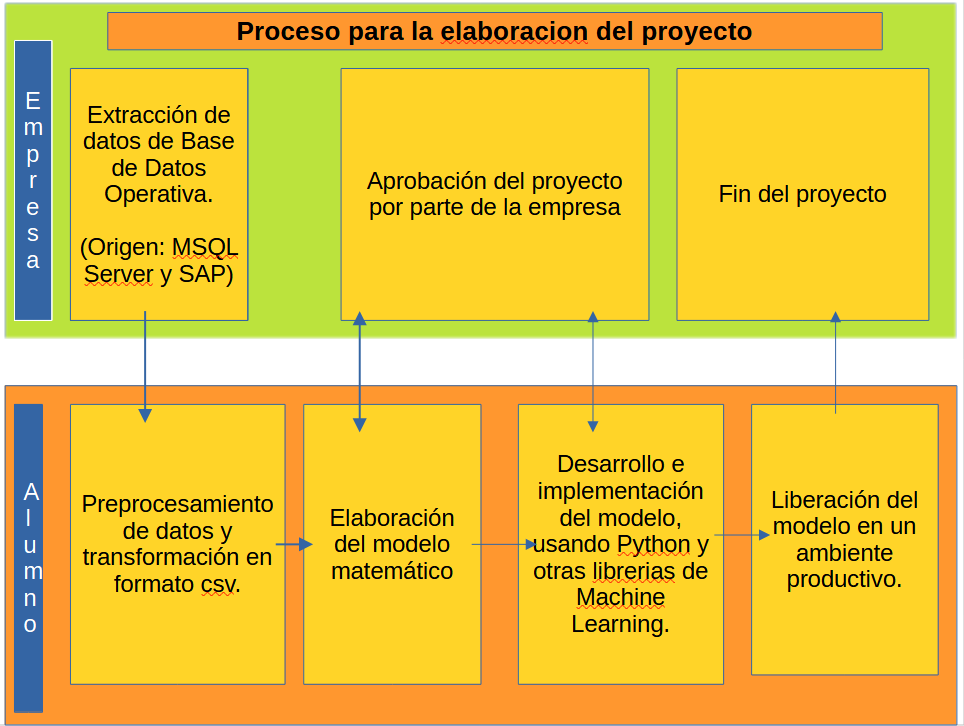
\includegraphics[width=12cm, height=7cm ]{Imagenes/Proceso_Proyecto.PNG }
      \caption{Metodología}
      \label{fig:meto}
\end{figure}

La metodología para realizar el proyecto se explica con la figura anterior.

\begin{itemize}
    \item La empresa proporciona la información con la que quiere que se desarrolle el modelo en formato Excel. \medskip
    \item Se recibe el archivo Excel y se realiza la limpieza y preprocesamiento de datos y se convierte a un formato de texto CSV , para usarlo como entrada por el algoritmo de aprendizaje . \medskip
    \item Se elabora el modelo y se interactúa con la empresa , hasta lograr un modelo este de acuerdo a sus necesidades. \medskip
    \item Una vez aprobado el modelo, se desarrolla el algoritmo usando el lenguaje de programación Python y otras librerías adicionales.\medskip
    \item El script o programa es evaluado por la empresa, la cual da su aprobación en cuanto a la funcionalidad requerida. \medskip
    \item Completado el anterior paso la empresa da su aprobación, con lo cual queda concluido el proyecto terminal. \medskip 
\end{itemize}

Una parte de dataset de trabajo es el siguiente :

\begin{figure}[H]
    \centering
       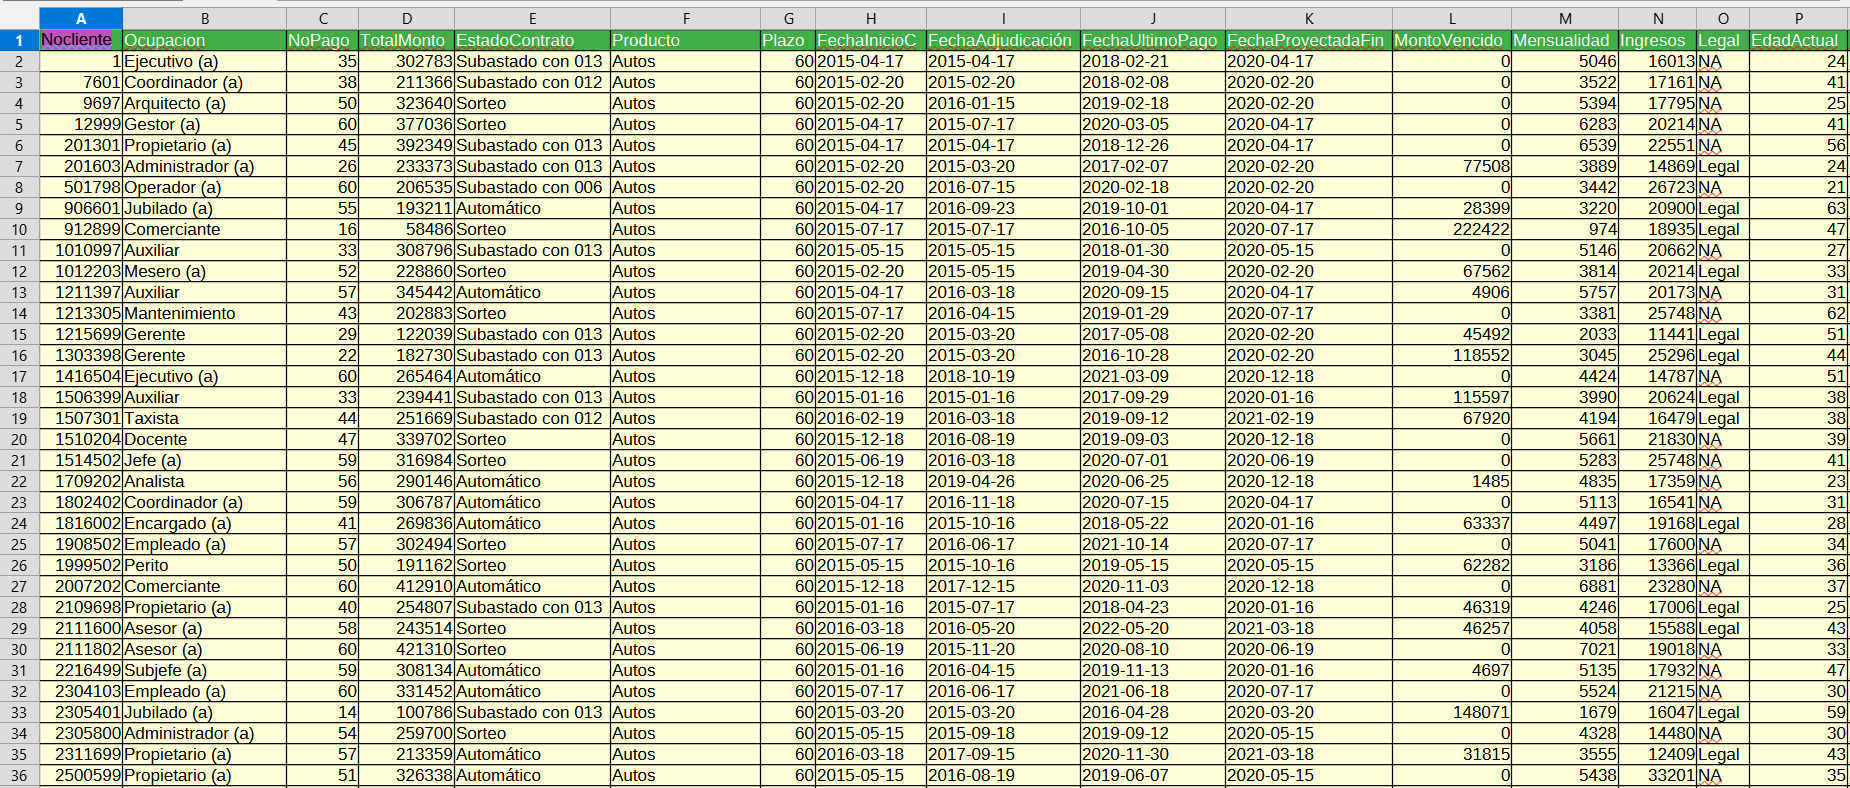
\includegraphics[width=16cm, height=10cm ]{Imagenes/Datos_Clientes1.PNG }
      \caption{Datos de los clientes (Bloque 1)}
      \label{fig:clis1}
\end{figure}
\newpage
\begin{figure}[H]
    \centering
       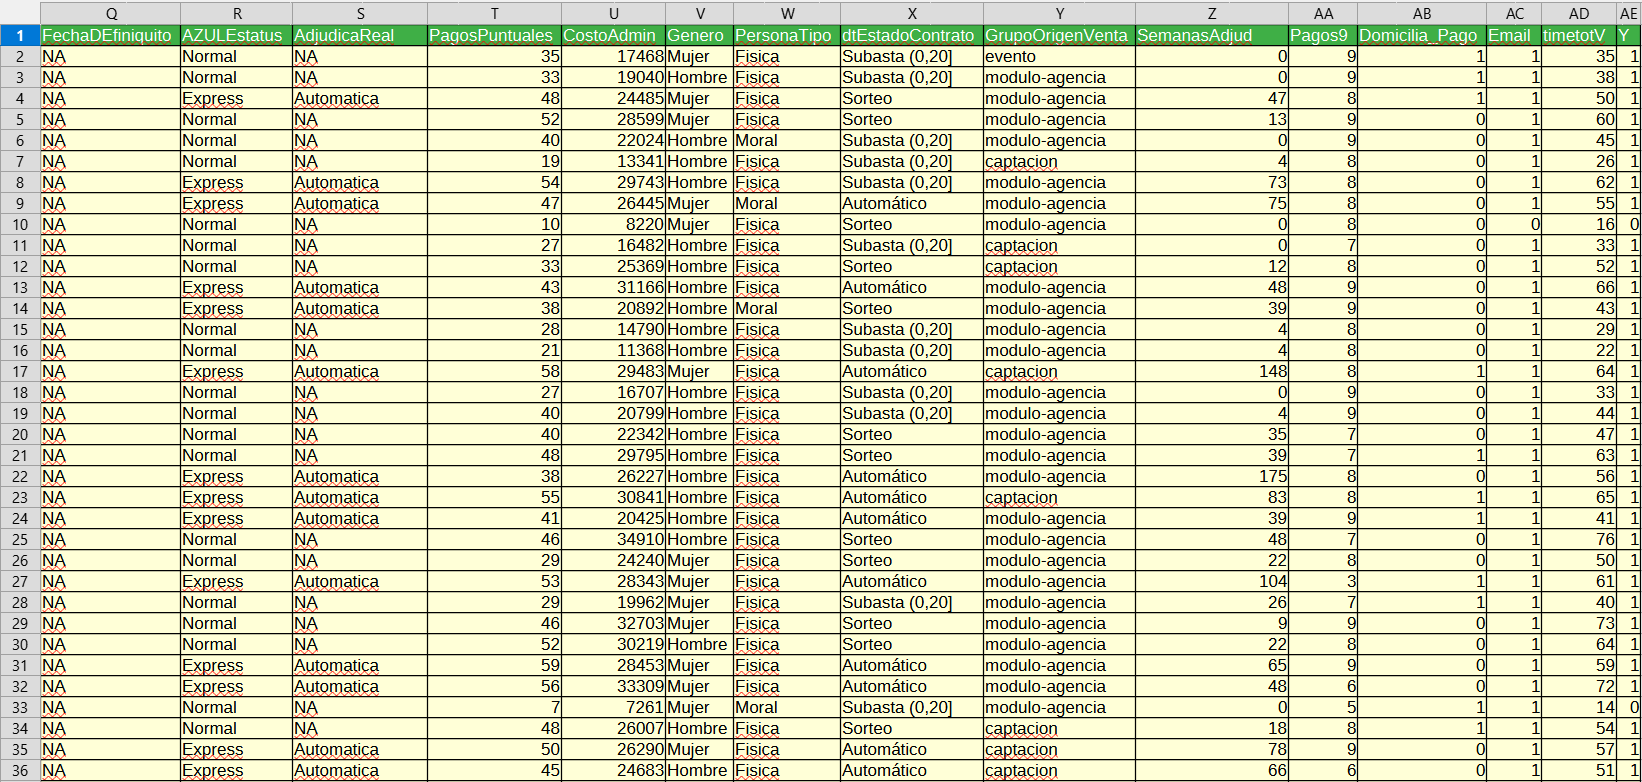
\includegraphics[width=16cm, height=10cm ]{Imagenes/Datos_Clientes2.PNG }
      \caption{Datos de los clientes (Bloque 2)}
      \label{fig:clis2}
\end{figure}
 
\section{Limpieza del dataset}

La limpieza de datos es una etapa esencial en el proceso de machine learning porque garantiza 
que el modelo trabaje con información de calidad, lo que mejora la precisión de sus resultados. 
Con frecuencia, los datos originales contienen errores, valores faltantes, duplicados o ruido, 
lo cual puede desviar el análisis y llevar a conclusiones equivocadas. Al procesar y limpiar los 
datos, se eliminan estas imperfecciones, ayudando a que el modelo se enfoque en patrones verdaderos
en lugar de anomalías. \medskip

La limpieza también permite identificar y gestionar los valores atípicos o outliers, que pueden 
distorsionar los resultados si no se manejan adecuadamente. Además, durante el proceso de 
limpieza, los datos se estandarizan y normalizan, especialmente cuando las variables presentan 
diferentes escalas o unidades; esto evita sesgos en el entrenamiento del modelo. \medskip

El programa o script para la limpieza de datos lo podemos ver en \cite{roh1} . \medskip

Comenzaremos viendo las variables categóricas del dataset con la instrucción Usando la libreria Pandas y 
Python\medskip
\begin{tcolorbox}[colback=gray!20, colframe=gray!80, width=\textwidth]
\begin{itemize}
\item datasetT.info()
\end{itemize}
\end{tcolorbox}
\newpage
Y obtenemos la siguiente información como respuesta

\begin{verbatim}
RangeIndex: 2000 entries, 0 to 1999 
Data columns (total 31 columns):
\end{verbatim}

\begin{table}[H]
    \centering
    \begin{tabular}{|c|c|c|c|c|}
        \hline
        \rowcolor{softblue} % Fila color azul suave
        \textbf{Num} & \textbf{Columna} & \textbf{Count} & \textbf{Non-Null} & \textbf{Dtype} \\
        \hline
        % \rowcolor{lightgray} % Fila color gris claro
        \hline
        0 &	Nocliente &		2000 &	non-null &	int64  \\
        \hline
        1 &	Ocupacion &		2000 &	non-null &	object \\
        \hline
        2 &  NoPago    &          2000 & non-null &  int64  \\
        \hline
        3 &  TotalMonto  &        2000 & non-null &  int64  \\
        \hline
        4 &  EstadoContrato &     2000 & non-null &  object \\
        \hline
        5 &   Producto  &         2000 & non-null &   object \\
        \hline
        6 &  Plazo     &          2000 & non-null &   int64  \\
        \hline
        7 &  FechaInicioC  &      2000 & non-null &   object \\
        \hline
        8 &  FechaAdjudicación &   2000 & non-null &   object \\
        \hline
        9 &   FechaUltimoPago &     2000 & non-null &   object \\
        \hline
        10 &  FechaProyectadaFin &  2000 & non-null &   object \\
        \hline
        11 &  MontoVencido &        2000 & non-null &   int64  \\
        \hline
        12 &  Mensualidad &         2000 & non-null &   int64  \\
        \hline
        \rowcolor{mediumgray}
        13 &  Ingresos &            1958 & non-null &   float64 \\
        \hline
        \rowcolor{mediumgray}
        14 &  Legal &               520 & non-null &    object \\
        \hline
        15 &  EdadActual &          2000 & non-null &   int64  \\
        \hline
        \rowcolor{mediumgray}
        16 &  FechaDEfiniquito &    0 & non-null &      float64 \\
        \hline
        17 &  AZULEstatus &         2000 & non-null &   object \\
        \hline
        \rowcolor{mediumgray}
        18 &  AdjudicaReal &        1457 & non-null &   object \\
        \hline
        19 &  PagosPuntuales &      2000 & non-null &   int64  \\
        \hline
        20 &  CostoAdmin &          2000 & non-null &   int64  \\
        \hline
        21 &  Genero &              2000 & non-null &   object \\
        \hline
        22 &  PersonaTipo &         2000 & non-null &   object \\
        \hline
        23 &  dtEstadoContrato &    2000 & non-null &   object \\
        \hline
        24 &  GrupoOrigenVenta &    2000 & non-null &   object \\
        \hline
        25 &  SemanasAdjud &        2000 & non-null &   float64 \\
        \hline
        26 &  Pagos9 &              2000 & non-null &   int64  \\
        \hline
        27 &  DomiciliaPago &      2000 & non-null &   int64  \\
        \hline
        28 &  Email &               2000 & non-null &   int64  \\
        \hline
        29 &  timetotV &            2000 & non-null &   int64  \\
        \hline
        30 &  Y &                   2000 & non-null &   int64 \\
        \hline  
    \end{tabular}
    \caption{Tabla con las variables numéricas y categóricas}
\end{table} \medskip
Esta tabla muestra que trabajaremos con un conjunto de datos de 2000 clientes y cada cliente con 30 columnas o variables. 
Además, nos indica la cantidad de información disponible en cada variable o columna. 
Si el tipo de dato (Dtype) es ''object'', la columna es categórica; de lo contrario, es una variable numérica.\medskip



Seguiremos los siguientes pasos \cite{Brown1} : \medskip
\begin{itemize}
    \item Eliminación de columnas con un único valor.
    \item Consideración de columnas con pocos valores únicos.
    \item Eliminación de columnas con baja variación.
    \item Identificación y eliminación de filas con datos duplicados.
    \item Eliminación de valores extremos (outliers) en caso de variables numéricas.
    \item Estandarización de errores tipográficos en variables categóricas.
\end{itemize}



\subsection{Eliminar columnas que contienen un solo valor} 

    La columna 'FechaDEfiniquito' no contiene información , ademas la columna 'Plazo' 
    solo tiene un valor por lo que las eliminamos con la 
    instruccion :
    \begin{tcolorbox}[colback=gray!20, colframe=gray!80, width=\textwidth]
        \begin{itemize}
            \item datasetT = datasetT.drop('FechaDEfiniquito', axis=1)
            \item datasetT = datasetT('Plazo', axis = 1)
        \end{itemize}
\end{tcolorbox}

\subsection{ Considerar y/o eliminar columnas que tienen muy pocos valores}

En este caso y con la información de la tabla anterior del dataset vemos que las columnas
'Ingresos' , 'Legal' y 'AdjudicaReal' tienen menos información por lo que la completaremos de
acuerdo con reglas de negocio de la empresa. \medskip

Completamos y corregimos estas columnas con las siguientes instrucciones \medskip

\begin{tcolorbox}[colback=gray!20, colframe=gray!80, width=\textwidth]
\begin{itemize}

\item datasetT['Ingresos'] = np.where((datasetT['Ingresos'] == 0) | (datasetT['Ingresos'].isnull()), datasetT['Mensualidad'] * 4, datasetT['Ingresos'])


\item datasetT['Legal'] = np.where((datasetT['Legal'] == 'NA') | (datasetT['Legal'].isnull()), 'Normal', datasetT['Legal'])


\item datasetT['AdjudicaReal'] = np.where((datasetT['AdjudicaReal'] == 'NA') | (datasetT['AdjudicaReal'].isnull()), 'Normal', datasetT['AdjudicaReal'])
\end{itemize}
\end{tcolorbox}

\subsection{ Identificar y eliminar filas duplicadas}

Dado que los clientes tienen un numero unico asignado, este proceso no se realiza. \medskip
\subsection{ Eliminación de valores extremos (outliers) en caso de variables numéricas}

En la siguiente tabla podemos ver los valores fuera de rango o outliers. \medskip

\begin{figure}[H]
    \centering
       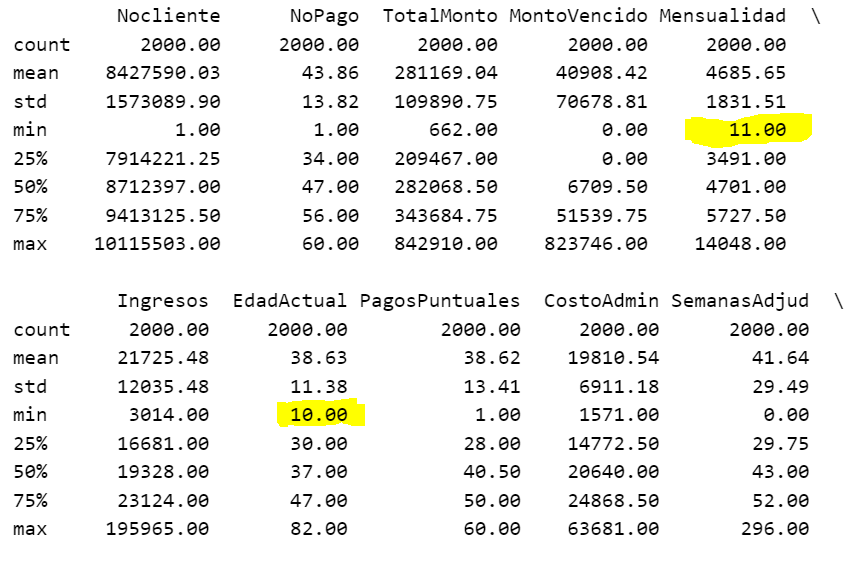
\includegraphics[width=16cm, height=10cm ]{Imagenes/Outliers.PNG }
      \caption{Valores fuera de rango o outliers}
      \label{fig:Outliers}
\end{figure}

En la tabla, se destaca en color amarillo la columna Mensualidad, la cual tiene un valor mínimo 
de 11 pesos. Por lo tanto, estos valores se incrementarán a 2,000 pesos. 
Además, la columna EdadActual presenta un valor mínimo de 10 años. 
Por ello, todos los valores menores de 18 años se ajustarán a 18 años. \medskip

Las instrucciones en Python y Pandas son :

\begin{tcolorbox}[colback=gray!20, colframe=gray!80, width=\textwidth]

    \begin{itemize}

        \item datasetT['Mensualidad'] = np.where((datasetT['Mensualidad'] <= 1999) | (datasetT['Mensualidad'].isnull()), 2000, datasetT['Mensualidad'])
        
        \item datasetT['EdadActual'] = np.where((datasetT['EdadActual'] <= 18) | (datasetT['EdadActual'].isnull()), 18, datasetT['EdadActual'])
        
    \end{itemize}

\end{tcolorbox}


 

\section{Analisis exploratorio del dataset}

\section{Transformación del dataset}

\section{Reducción de dimensionalidad}

\subsection{SVD}
\subsection{PCA}

\section{Partición del dataset}

    \begin{figure} [H]
        \centering
        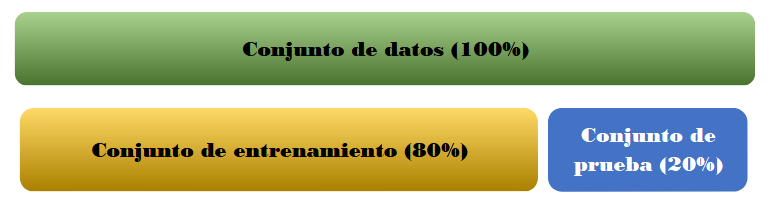
\includegraphics[width=12cm, height=4cm ]{Imagenes/ParticionDEdatos.PNG }
        \caption{Partición del dataset}
        \label{fig:parti}
    \end{figure}

\section{Partición del dataset}



